\documentclass[a4paper,man,natbib]{apa6}

\usepackage[english]{babel}
\usepackage[utf8x]{inputenc}
\usepackage{amsthm}
\usepackage{amsmath}
\usepackage{amssymb}
\usepackage{mathtools}
\usepackage{graphicx}
\usepackage[colorinlistoftodos]{todonotes}
\usepackage{url}

\newcommand{\C}{\mathbb{C}}  % Complex
\newcommand{\R}{\mathbb{R}}  % Real
\newcommand{\Q}{\mathbb{Q}}  % Rational
\newcommand{\Z}{\mathbb{Z}}  % Integers

\title{Betweenness of Undirected Graphs}
\shorttitle{Betweenness}
\author{$ \C $ason Konzer}
\date{April 2021}
\affiliation{University of Michigan \\ Mathematics}

\abstract{In this paper we will review the axiomatic theory of betweenness described in the referenced article. 
The outline starts with background material, followed by a summary of the article. 
After the setting is in place, we will speak to areas that were hard to understand and those that were straight forward.
Ideas that are new and intresting will be explored and those that are troubling we will question and add suguestion. 
At this point the paper will be well explained and we will take the time to do a deep dive into a proof or two and end with an extension to the ideas presented.\\
\textbf{Keywords:} Betweenness, Axioms, Undirected Graph, Region, Path, Point.}

\begin{document}
\maketitle

\section{Background \& Summary}
\label{sec: The Lay of The Land}
      Azimipour and Naumov begin their article, \textit{Axiomatic theory of betweenness}, with the discussion of betweenness of points. 
The idea of betweenness is in it's simpiliest form when concering points on a line, but this idea can be generalized to many other structures. 
Structures of points on a plane are mentioned, used connected paths rather than lines, and graphs concerning betweenness of verticies in relation to internal verticies. 
Betweenness is then laid out for sets of objects before reviewing the insertion principle. At this time it is relevant to list a few defintions we will continue to reference throughout this paper.

\begin{itemize}

      \item \underline{Point}: A point is a uniquely determined location in space quantifiable by one or more reference variables. 

      \item \underline{Vertex}: Verticies are the fundamental building blocks of graphs, they are thought of as a possible point accessible within a graph.

      \item \underline{Path}: A path is a mode of transportation between points, or verticies alike, paths can be defined as directional or undirectional, thought of one-way or two-way roads.

      \item \underline{Line}: A line is a specific type of path that has no curvature with repect to all of it's variables. Lines are characterized as being "straight."

      \item \underline{Edge}: An edge is simply a path between two verticies within a graph. For our discussion, edges do not have to be lines. 

      \item \underline{Multiple Edges}: A graph that is defined as having multiple edges is a graph that that has more than one edge connecting any two verticies.
      
      \item \underline{Set}: A set is a collection of objects. These objects can take many different forms; for instance: points, verticies, edges, etc. 

      \item \underline{Directed}: A directed line or path, is a transition from one point, to another, in which can only be traversed one way
      For instance, if there are two points, $ a $ and $ b $, a directed path from $ a $ to $ b $ cannot be traversed from $ b $ to $ a $. An undirected path can be traversed in either direction. 

      \item \underline{Undirected Graph}: An undirected graph is a collection of edges and verticies, in which every edge can be travered in either direction. 

      \item \underline{Internal Point}: A point, $ p $, is considered internal given that on some path between two points, $ p_i $ and $ p_f $ traverses $ p $ in both directions. 

      \item \underline{Internal Vertex}: An internal vertex in analagous to an internal point given the path is an edge between two verticies,  $ v_i $ and $ v_f $, with a vertex $ v $ inbetween. 

      \item \underline{Between}: As mentioned in the context of an internal vertex; An object is considered between two other objects, given it is an internal object. 

      \item \underline{Axiom}: An axiom is a fundamental law/idea that is taken to be self evident. Axioms are the building blocks for proofs and mathematical theory. It is from axioms that theorems are derived.
      
\end{itemize}

\noindent
To understand the insertion principle, we must first come to the realization that given any two unique points, there exists a thrid point that is between them. 
This has a great deal of extensions, and a very intresting one mentioned is that there is always a rational number between a rational and an irrational. 
Using the notation from the article, this is written as $ \Q | \Q | \R \backslash \Q $. 
In gernal the notation for an object $ B $ between $ A $ and $ C $ is given by, $ A | B | C $. 
From here the authors take a moment to describe the insertion principle and some of the conesquences that follow from it. 
Very similar to transitivity the insertion principle is stated that notationally \dots

\begin{center}

      $ ( ( (A | B | C) \land (A | I | B) ) \implies (A | I | C) ) $, or $ ( (A | B | C) \implies( (A | I | B) \implies (A | I | C) ) ) $. 

\end{center}

\noindent
From this we can see that it is relatively obvious that when one point, $ I $, is between a point $ A $, and a point $ B $, that is inbetween $ A $, and $ C $, then $ I $ is also between the same two points, $ A $, and $ C $.
Figure 1 is avaliable for a graphical representation of this principal. It is now relevant to realize that the notation used for betweenness exhibits a symmetry as $  (A | B | C) \equiv (C | B | A) $. 
This symmetry holds for undirected graphs as this is the same as saying that $ B $ is between both the paths $ \overrightarrow{AC} $ and $ \overrightarrow{CA} $. 
The following realization from exploring the insertion principle is that there are even stronger forms of the principle. 
The main point of the article is thus to prove that the following insertion principle \dots 

\begin{center}

      $ (A | B_1 , I , B_2 | C) \implies ((A | I , C | B_1) \implies ((B_2 | A , I | C) \implies (A | I | C ))) $ 

\end{center}

\noindent
Is the strongest possible definition of the insertion principle with respect to undirected graphs, without any instances of multiple edges. 
Here a comma butween two objects is thought of as the unioned set containing either both of the objects, or both of the sets of objects. ($ (B_1 , I , B_2) \equiv (B_1 \cup I \cup B_2) $). 
It follows that this same principal holds for arbitrarily closed sets witin a topological space. 
Here $ A , B , C $ are either verticies or closed sets. The authors outline the proof and follow with a formalization of syntax and semantics. 
An axiomatic approach is taken within this encapusalting proof, Thus the authors next outline the axioms needed. 
Lastly each axiom implies finite graphs, know as soundness, and then the converse such that any finite graph implies each axiom, know as completness. 
Once both soundness and completeness are proven, each axiom, including insertion, is considered biconditional for finite graphs, thus verifying their postulate.  
The authors seem very intrigued by the subject of betweenness and are not reluctant to mention different variations of the postulate, or the applications of it's study. 
With the general audience being mathematics students, advocates, and researchers; 
The author's main point of the article is to present a well defined and in depth proof while inspiring further study of betweenness.


\section{Betweenness}
\label{sec:Graphs and Points}

\subsection{A Visual Look}
As a very visual thinker, the graphs produced by the authors were very helpful in my understanding of the presented concepts.
With this said the topic of insertion was the last moment where graphs were used, and a more in depth depiction is granted. 
Here I take the strong insertion principal and represent the argument in terms of both undirectional graphs as well as closed sets. 
To break down the principal, we must look at each assumption step by step. Listed are the assumptions in order \dots

\begin{enumerate}

      \item $ A | B_1 \cup I \cup B_2 | C $

      \item $ A | I \cup C | B_1 $

      \item $ B_2 | A \cup I | C $

      \item $ A | I | C $

\end{enumerate}

\noindent
In particular, 4., Is the conclusion of the first three assumptions that must be proven. 
What was most helpful to me was the visualization of these assumptions. 
Figure 2 and Figure 3 provide a drawn representation in terms of verticies and closed sets. 
As a result of this exploration, the collorary that $ B_1 | I | B_2 $ became self evident.
This results as \dots 

\begin{center}

      $ (((A | I | C) \land (B_2 | A \cup I | C)) \implies (B_2 | I | C)) $ \\
      $ (((A | I | C) \land (A | I \cup C | B_1)) \implies (A | I | B_1)) $ \\
      From here it follows \dots \\
      $ (((B_2 | I | C) \land (A | I | B_1)) \implies (B_2 | I | B_1)) \implies (B_1 | I | B_2) $ \\
      * Figure 4 illustrates these paths.

\end{center}

This was a nice consequence and it drove inspiration to visualize the remaining axioms presented. 
The first few are quite trivial and are illustrated in Figure 5. 
The trivial path axiom simply states that there is nothing inbetween two sets, given they share an object. 
This is because there will always be the path from the object to itself, virtually then traveling between the two sets.
The empty set is vacuously true as you must travel through some set to get to another set from nowhere. 
Here the between set is a virtual starting point. 
The shortest path axiom states that the quickest route to a set is from the boundary of the first, given there is a set inbetween the two. 
This makes sense as you are virtually starting from a point inbetween the two sets. 
Lastly symmetry is held as previously defined. 
Moving onto the more complex axioms, aggregation is quite intuitive as if something is between two sets, it should also be between their union. 
Transitivity follows as if there is no path from two different sets to an element, such that the path passes some other inbetween set, then there should also be no path between the two different sets such that it must past through some inbetween set.
The last axioms of monotonicity are fairly less intuitive and seem to be defined with a choice of preference. These axioms define how we deal with unioned sets either between two sets or that have a set between their union and some other set.
Similarly these axioms are illustrated in Figure 6. 




\subsection{Favorite Proof and Confusion}

      Of these many proofs within this article, the soundness of insertion is by far the proof I found most appealing.
The proof goes as following.

\begin{proof}[\textbf{Proof}]

      Assume the following:

      \begin{itemize}

            \item there exist elements $ a $ \& $ c $ such that $ a \in A $ \& $ c \in C $, the outer sets.
      
            \item $ \gamma $ is a path between 2 elements $ a $ \& $ c $ such that the path traverses from $ e_0 $ to $ e_f $ where $ e_0 = a $ \& $ e_f = c $.
      
            \item $ e_i = i $ be an inserted element such that $ i \in I $, the inserted sets. 
      
            \item $ i $ is not between $ a $ \& $ c $, therfore the index $ i $ is some number such that $ 0 \nleq i \nleq f $, or $ f < i < 0 $.
      
            \item $ e_a $ is the last indexed element on the path $ \gamma $ such that the element is a member of $ A $ \& $ e_a \neq e_0 $
            \item $ e_c $ is the first indexed element on the path $ \gamma $ such that the element is a member of $ C $ \& $ e_c \neq e_f $

      \end{itemize}

      \noindent
      From these assumptions we will prove insertion by contradiction. 
      The first thing to notice is that the indexed elements $ e_{a+1} \to e_{c-1} $ are all elements outside of the set $ A \cup I \cup C $. 
      The insertion principle, $ A | B_1 \cup I \cup B_2 | C $, can now be reduced to $ A | B_1 \cup B_2 | C $. 
      This then implies that there is some element $ e_b $ such that $ e_b \in B_1 \cup B_2 $ given that the index $ b $ obeys $ a < b < c $. 
      From the axiom of central monotonicity we can then assume that $ e_b \in B_1 $. 
      Simplifying our betweenness relation, we can now see $ A | B_1 | C $.
      Again referensing the insertion principal, we now take the second assumption that $ A | I \cup C | B_1 $.
      It should now be obvious that we have reached a contradiction. 
      $ B_1 $ is between $ A $ \& $ C $, therefor $ C $ is not between $ A $ \& $ B_1 $ which implies $ A | I | B_1 $. 
      The problem is that we know the index $ i $ is such that $ 0 \nleq i \nleq f $ \& $ a \nleq i \nleq c $, therefore $ a \nleq i \nleq b $ as $ a < b < c $.
      This contradiction concluded the proof of insersion, thus $ 0 < i < f $.

\end{proof}

      On the other hand there were a few proofs and definitions that left me confused in this reading. 
In general, the assumptions for the completeness proofs could've used a more verbal definition. 
One question I have is, "What additional axioms X are used when defining completeness?"
Overall this was a very intresting paper that I will be saving to read again at a later date. 

\newpage
\subsection{References}

      Azimipour, S., Naumov, P. Axiomatic theory of betweenness. Arch. Math. Logic 60, 227–239 (2021). 
\url{https://doi.org/10.1007/s00153-020-00744-5}


% Commands to include a figure:

\begin{figure}

      \centering
      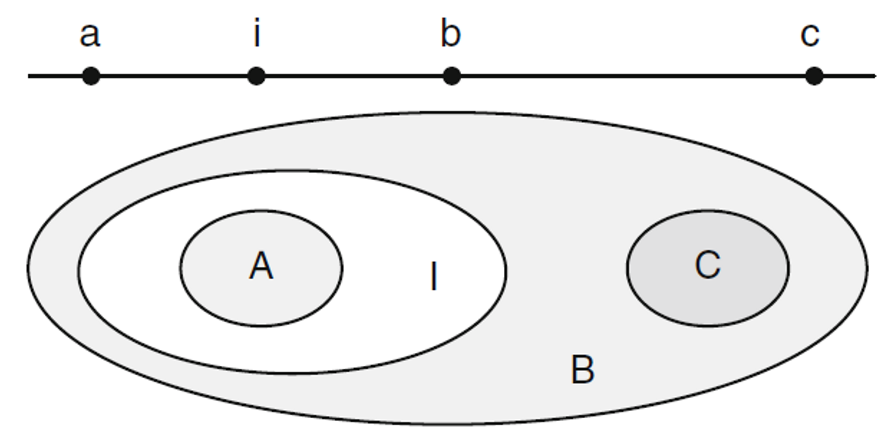
\includegraphics[width=1\textwidth]{C:/Users/cason/OneDrive - Umich/Math/PS/Betweenness Research/Insertion.png}
      \caption{\label{C:/Users/cason/OneDrive - Umich/Math/PS/Betweenness Research/Insertion.png}
      Illustrated here is a graphical representation of the insertion principal for both a line and for set. Sourced- (Azimipour, Naumov. 2021).}

\end{figure}

\begin{figure}

      \centering
      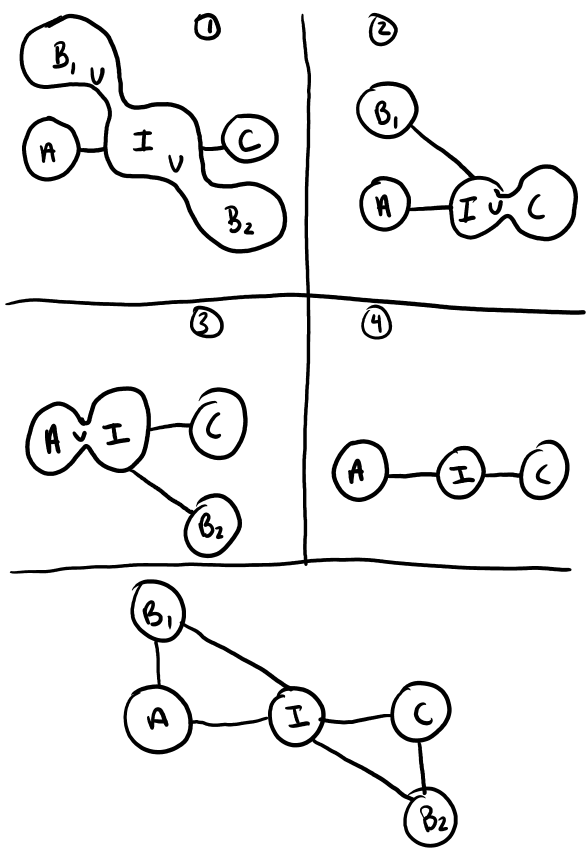
\includegraphics[width=1\textwidth]{C:/Users/cason/OneDrive - Umich/Math/PS/Betweenness Research/Vert-Insert.png}
      \caption{\label{C:/Users/cason/OneDrive - Umich/Math/PS/Betweenness Research/Vert-Insert.png}
      Illustrated here is a graphical representation of the strong insertion principal with respect to verticies.}

\end{figure}

\begin{figure}

      \centering
      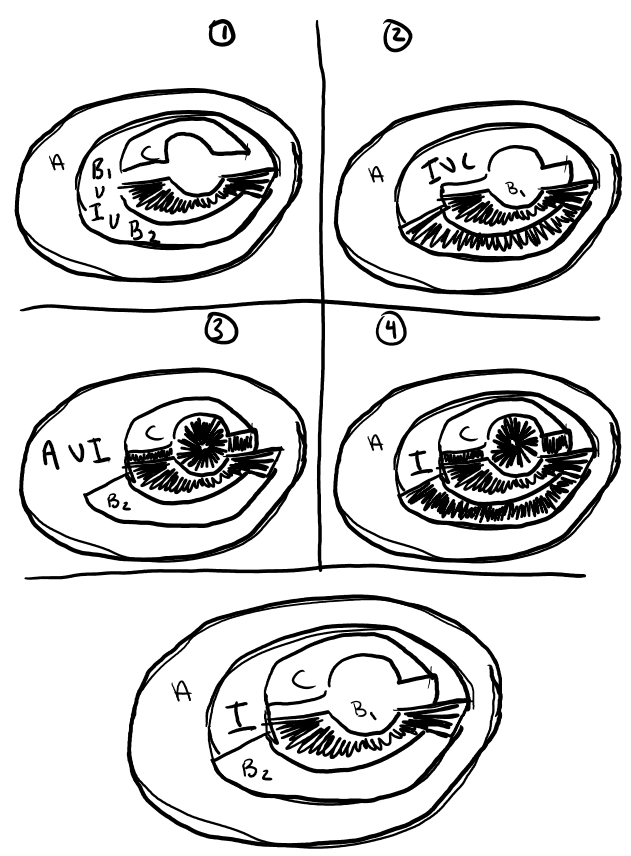
\includegraphics[width=1\textwidth]{C:/Users/cason/OneDrive - Umich/Math/PS/Betweenness Research/Set-Insert.png}
      \caption{\label{C:/Users/cason/OneDrive - Umich/Math/PS/Betweenness Research/Set-Insert.png}
      Illustrated here is a graphical representation of the strong insertion principal with respect to closed sets. The dark areas can be though of as empty sets.}

\end{figure}

\begin{figure}

      \centering
      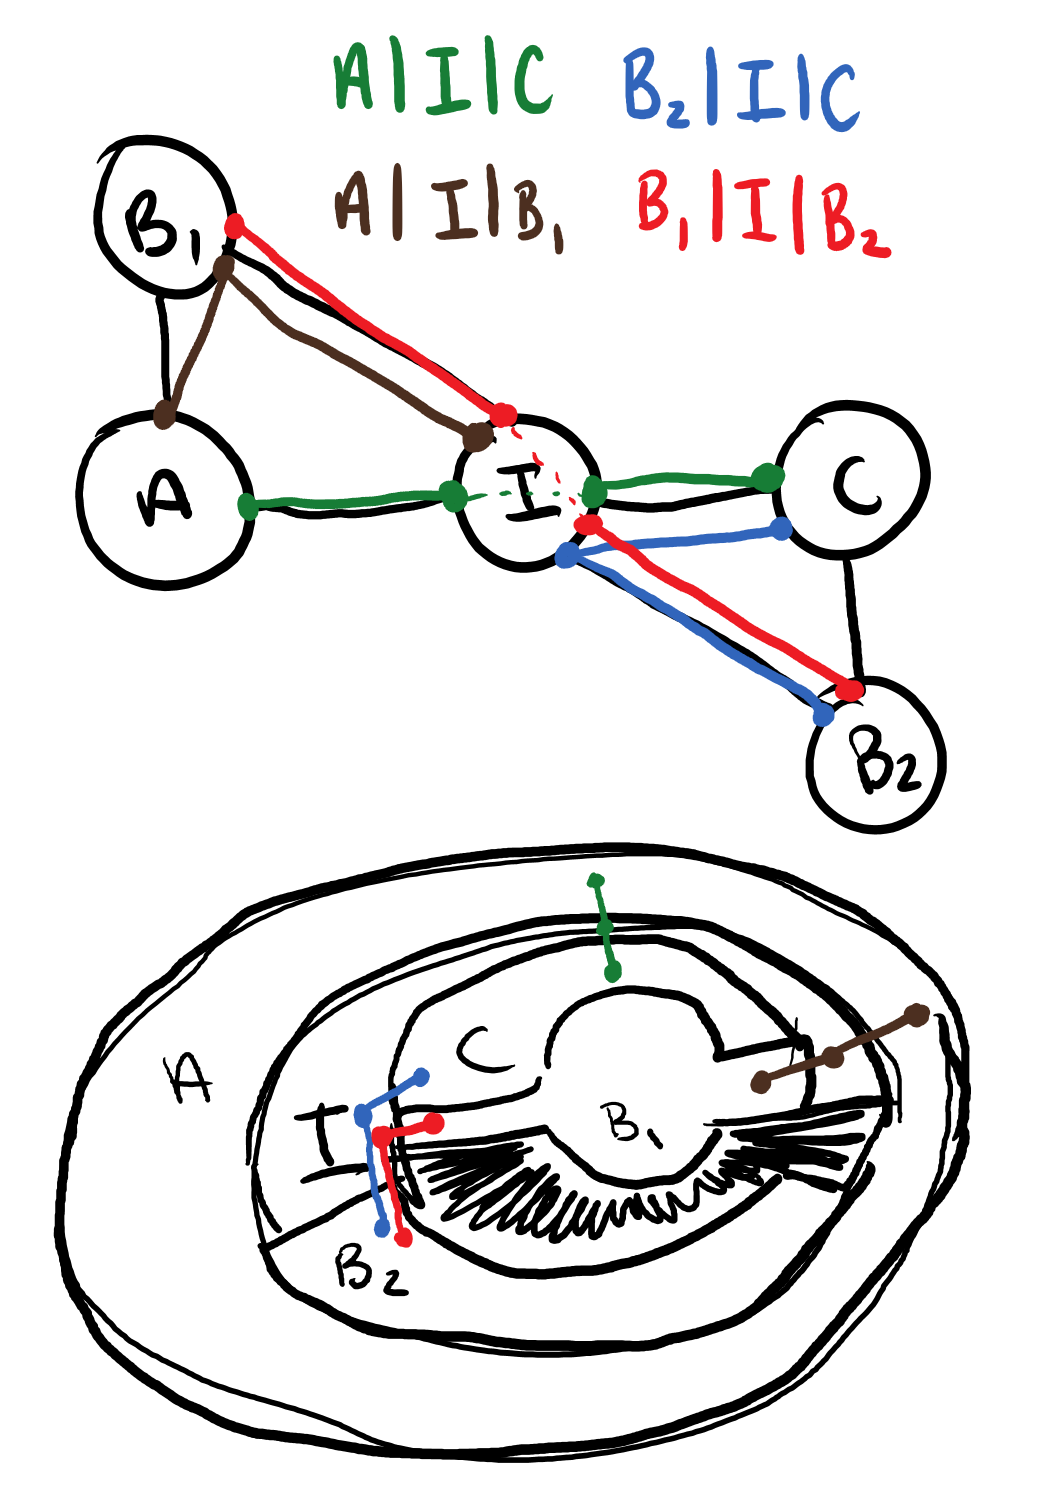
\includegraphics[width=1\textwidth]{C:/Users/cason/OneDrive - Umich/Math/PS/Betweenness Research/Collorary.png}
      \caption{\label{C:/Users/cason/OneDrive - Umich/Math/PS/Betweenness Research/Collorary.png}
      Illustrated here is a graphical representation of the collorary consequence of strong insertion.}

\end{figure}

\begin{figure}

      \centering
      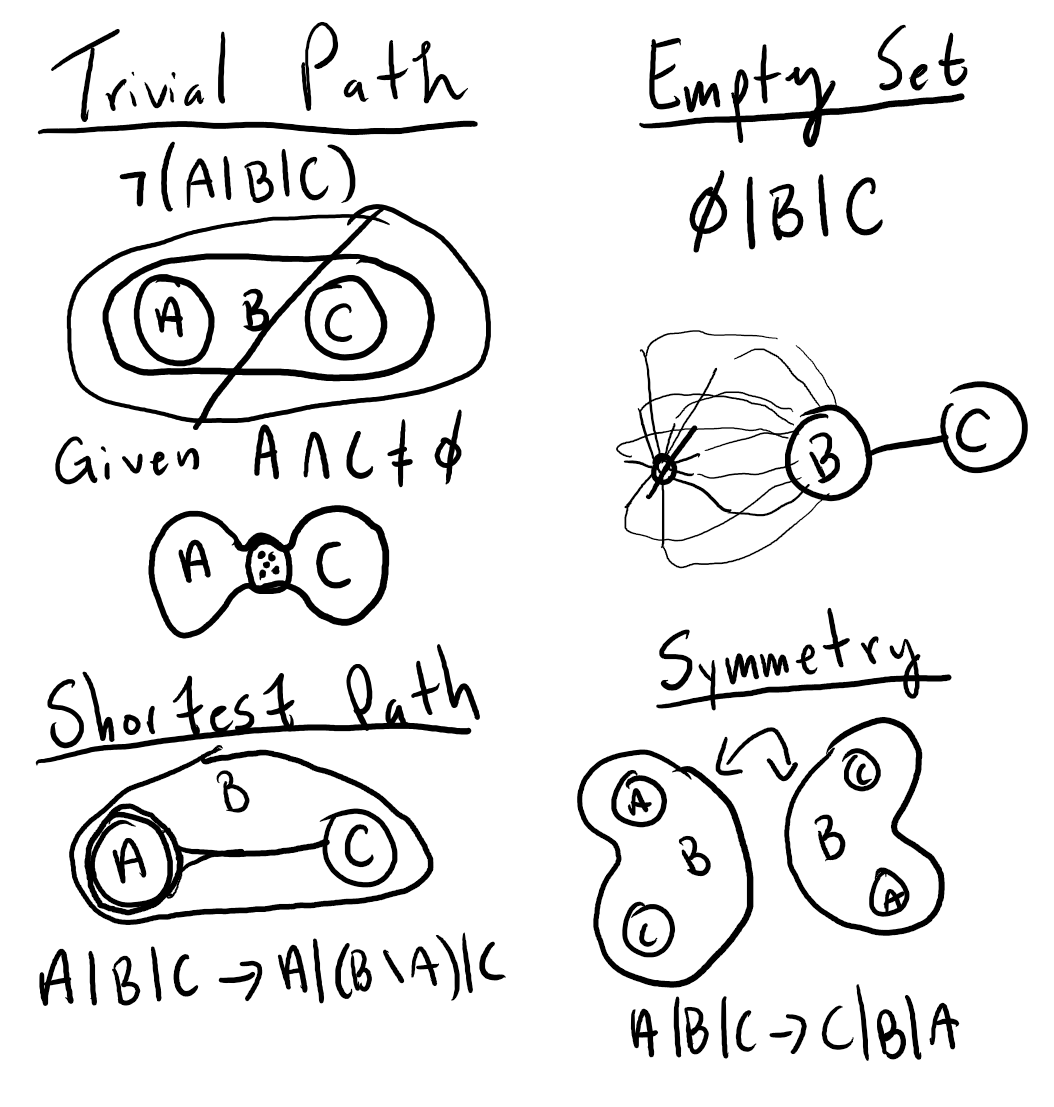
\includegraphics[width=1\textwidth]{C:/Users/cason/OneDrive - Umich/Math/PS/Betweenness Research/Trivial.png}
      \caption{\label{C:/Users/cason/OneDrive - Umich/Math/PS/Betweenness Research/Trivial.png}
      Illustrated here is are the first trivial axioms of betweenness.}

\end{figure}

\begin{figure}

      \centering
      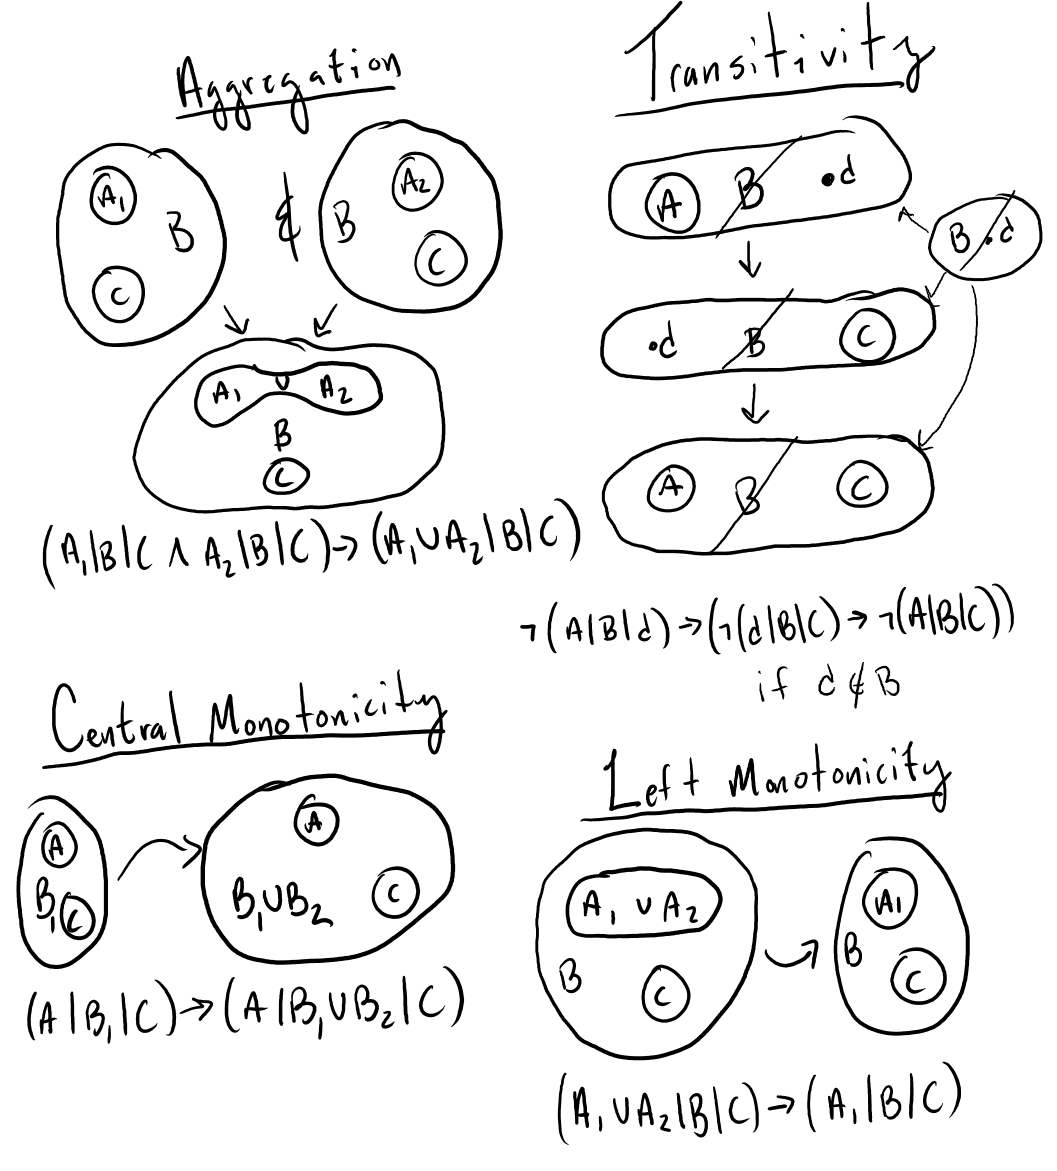
\includegraphics[width=1\textwidth]{C:/Users/cason/OneDrive - Umich/Math/PS/Betweenness Research/Axioms.png}
      \caption{\label{C:/Users/cason/OneDrive - Umich/Math/PS/Betweenness Research/Axioms.png}
      Illustrated here is are the less intuitive axioms of betweenness.}

\end{figure}

\end{document}

%Comments - April 2021 Proofs and Structures Paper%